\addcontentsline{toc}{chapter}{Appendices}



% The \appendix command resets the chapter counter, and changes the chapter numbering scheme to capital letters.
%\chapter{Appendices}
\appendix
\chapter{Tully Model Paramters}
\label{ap:tully_params}

\section{Model 1 -Single Avoided Crossing}
  \begin{minipage}{0.5\textwidth}
      \textbf{Hamiltonian Paramters:}
      \begin{flalign*}
        H_{11}(\mathbf{R}) \ &= \ A \ \tanh(B\mathbf{R}) &\\
        H_{12}(\mathbf{R}) \ &= \ C e^{-D\mathbf{R}^2} \\
        H_{21}(\mathbf{R}) \ &= \ H_{12}(\mathbf{R}) \\
        H_{22}(\mathbf{R}) \ &= \ -H_{11}(\mathbf{R})
      \end{flalign*}
      Where A = 0.03, B = 0.4, C = 0.005 and D = 0.3
  \end{minipage}
  \hspace{0.5cm}
  \vrule
  \hspace{0.5cm}
  \begin{minipage}{0.6\textwidth}
      \begin{tabular}{l|l|c}
        \textbf{Quantity} & \textbf{Value} & \textbf{Unit} \\
        \hline
        Initial Position & -20 & a.u. \\
        Initial Velocities & 15.0, 25.0 & a.u. \\
        Initial Adiab Pop & ground state & - \\
        Simulation Time & 6000, 4000 & a.u. \\
        $\sigma_{\nu}^{(I)}$ & 0.5 & a.u. \\
        M ($\sigma$ constant) & 40 & - \\
        $\Delta t_{\text{nuclear}}$ & 0.1 & fs \\
        $\Delta t_{\text{electonic}}$ & 0.01 & fs \\
        $\frac{\delta \mathbf{R}_{lk, \nu}^{(I)}}{\delta t}$ threshold & 0.15 & a.u. \\
        N$_{rep}$ & 200 & - \\
      \end{tabular}
  \end{minipage}

\section{Model 2 -Dual Avoided Crossing}
\begin{minipage}{0.48\textwidth}
    \textbf{Hamiltonian Paramters:}
    \begin{flalign*}
      H_{11}(\mathbf{R}) \ &= \ 0 &\\
      H_{12}(\mathbf{R}) \ &= \ C e^{-D \mathbf{R}^2} \\
      H_{21}(\mathbf{R}) \ &= \ H_{12}(\mathbf{R}) \\
      H_{22}(\mathbf{R}) \ &= \ -A e^{-B\mathbf{R}^2} + E
    \end{flalign*}
    Where A = 0.1, B = 0.28, C = 0.015, D = 0.06 and E = 0.05
  \end{minipage}
  \hspace{0.5cm}
  \vrule
  \hspace{0.5cm}
  \begin{minipage}{0.6\textwidth}
      \begin{tabular}{l|l|c}
        \textbf{Quantity} & \textbf{Value} & \textbf{Unit} \\
        \hline
        Initial Position & -8 & a.u. \\
        Initial Velocities & 16.0, 30.0 & a.u. \\
        Initial Adiab Pop & ground state & - \\
        Simulation Time & 2500, 1500 & a.u. \\
        $\sigma_{\nu}^{(I)}$ & 0.5 & a.u. \\
        M ($\sigma$ constant) & 40 & - \\
        $\Delta t_{\text{nuclear}}$ & 0.1 & fs \\
        $\Delta t_{\text{electonic}}$ & 0.01 & fs \\
        $\frac{\delta \mathbf{R}_{lk, \nu}^{(I)}}{\delta t}$ threshold & 0.15 & a.u. \\
        N$_{rep}$ & 200 & - \\
      \end{tabular}
  \end{minipage}

\section{Model 3 -Extended Coupling}
\begin{minipage}{0.5\textwidth}
    \textbf{Hamiltonian Paramters:}
    \begin{flalign*}
      H_{11}(\mathbf{R}) \ &= \ A  &\\
      H_{12}(\mathbf{R}) \ &= \ \left \lbrace
      \begin{array}{l}
        B e^{C\mathbf{R}}, \qquad \qquad R \leq 0 \\
          B(2 - e^{-C\mathbf{R}}), \quad R > 0\\
      \end{array} \right . \\
      H_{21}(\mathbf{R}) \ &= \ H_{12}(\mathbf{R}) \\
      H_{22}(\mathbf{R}) \ &= \ -H_{11}(\mathbf{R})
    \end{flalign*}
    Where A = 6$\times$ 10$^{-4}$, B = 0.1 and C = 0.9
  \end{minipage}
  \hspace{0.2cm}
  \vrule
  \hspace{0.6cm}
  \begin{minipage}{0.6\textwidth}
      \begin{tabular}{l|l|c}
        \textbf{Quantity} & \textbf{Value} & \textbf{Unit} \\
        \hline
        Initial Position & -15 & a.u. \\
        Initial Velocities & 10, 30 & a.u. \\
        Initial Adiab Pop & ground state & - \\
        Simulation Time & 5000, 1500 & a.u. \\
        $\sigma_{\nu}^{(I)}$ & 0.5 & a.u. \\
        M ($\sigma$ constant) & 40 & - \\
        $\Delta t_{\text{nuclear}}$ & 0.1 & fs \\
        $\Delta t_{\text{electonic}}$ & 0.01 & fs \\
        $\frac{\delta \mathbf{R}_{lk, \nu}^{(I)}}{\delta t}$ threshold & 0.15 & a.u. \\
        N$_{rep}$ & 200 & - \\
      \end{tabular}
  \end{minipage}


\section{Model 4 -Dual Arch}
\hspace*{-1.5cm}
\begin{minipage}{0.49\textwidth}
    \textbf{Hamiltonian Paramters:}
    \begin{flalign*}
      H_{11}(\mathbf{R}) \ &= \ A  &\\
      H_{12}(\mathbf{R}) \ &= \ \left \lbrace
      \begin{array}{l}
        B \left[ -e^{C(\mathbf{R} - D)} + e^{C(\mathbf{R} + D)} \right] \ \qquad \qquad \ R \leq -D \\
        B \left[ e^{-C(\mathbf{R} - D)} - e^{-C(\mathbf{R} + D)} \right] \ \ \ \ \ \qquad \quad R \geq D \\
        B \left[ 2 - e^{C(\mathbf{R} - D)} - e^{-C(\mathbf{R} + D)} \right] \ \ -D < R < D \\
      \end{array} \right . \\
      H_{21}(\mathbf{R}) \ &= \ H_{12}(\mathbf{R}) \\
      H_{22}(\mathbf{R}) \ &= \ -H_{11}(\mathbf{R})
    \end{flalign*}
    Where A = 6$\times$ 10$^{-4}$, B = 0.1, C = 0.9 and D = 4
  \end{minipage}
  \hspace*{-0.2cm}
  \vrule
  \hspace{0.2cm}
  \begin{minipage}{0.6\textwidth}
      \begin{tabular}{l|l|c}
        \textbf{Quantity} & \textbf{Value} & \textbf{Unit} \\
        \hline
        Initial Position & -20 & a.u. \\
        Initial Velocities & 10, 40 & a.u. \\
        Initial Adiab Pop & ground state & - \\
        Simulation Time & 6000, 2000 & a.u. \\

        $\sigma_{\nu}^{(I)}$ & 0.5 & a.u. \\
        M ($\sigma$ constant) & 40 & - \\
        $\Delta t_{\text{nuclear}}$ & 0.1 & fs \\
        $\Delta t_{\text{electonic}}$ & 0.01 & fs \\
        $\frac{\delta \mathbf{R}_{lk, \nu}^{(I)}}{\delta t}$ threshold & 0.15 & a.u. \\
        N$_{rep}$ & 200 & - \\
      \end{tabular}
  \end{minipage}
















\chapter{Wigner Distribution Derivation}
\label{ap:Wigner}
The nuclear wavepacket (at time 0) is given by:
\begin{equation}
  \chi(R) = \frac{1}{(\pi \mu^2)^{\frac{1}{4}}} e^{-\frac{(R - R_0)^2}{2 \mu^2} + \im k_0 (R - R_0) }
  \label{eq_ap:initial_nucl_wp}
\end{equation}
The Wigner quassiprobability function for momentum and position (p, R) is given by:
\begin{equation}
  W(p, R) = \frac{1}{\pi \hbar} \int_{-\infty}^{\infty} \chi^{*}(R + y) \chi(R -y) e^{\frac{2 \im p y}{\hbar}} dy
  \label{eq_ap:Wig_def}
\end{equation}
However, both Ehrenfest and CTMQC require atomic positions as input so we must extract the position and velocity probability densities from this. We get these from the marginal integrals of the Wigner distribution i.e.
\begin{equation}
  \vert f(R)\vert^2 = \int^{\infty}_{-\infty} W(R, p) dp
\end{equation}
\begin{equation}
  \vert f(p)\vert^2 = \int^{\infty}_{-\infty} W(R, p) dR
\end{equation}
In order to calculate these marignal integrals we must first crunch through the maths of equation \eqref{eq_ap:Wig_def}. Substituting eq \eqref{eq_ap:initial_nucl_wp} into \eqref{eq_ap:Wig_def}:
\begin{equation}
  W(p, R) = \frac{1}{\pi \hbar} \int_{-\infty}^{\infty} \frac{1}{\mu \sqrt{\pi}} e^{- \frac{(R + y - R_0)^2}{2 \mu^2} - 2\im k_0y - \frac{(R - y - R_0)^2}{2 \mu^2} } e^{\frac{2 \im p y}{\hbar}} dy
  \label{eq_ap:step1}
\end{equation}
Simplifying the 2 quadratic equations (equation \eqref{eq_ap:step1}) we get:
\begin{equation}
  W(p, R) = \frac{1}{\pi \hbar} \int_{-\infty}^{\infty} \frac{1}{\mu \sqrt{\pi}} e^{-\mu^{-2} \left(y^2 - 2\im k_0y \mu^2 + (R - R_0)^2 \right) } e^{\frac{2 \im p y}{\hbar}} dy
  \label{eq_ap:step2}
\end{equation}
We can now take the expressions not dependant on y outside of the integral and combine the exponents.
\begin{equation}
  W(p, R) = \frac{1}{\pi \sqrt{\pi} \mu \hbar} e^{-\frac{(R - R_0)^2}{\mu^2}} \int_{-\infty}^{\infty} e^{-\frac{y^2 + 2 \im y\mu^{2}\left( \frac{p}{\hbar} - k_0\right)}{\mu^{2}}  } dy
  \label{eq_ap:step3}
\end{equation}
Integrating we get:
\begin{equation}
  \int e^{-\frac{y^2 + 2 \im y\mu^{2}\left( \frac{p}{\hbar} - k_0\right)}{\mu^{2}}  } dy = \frac{\sqrt{\pi} \mu}{2} e^{-\frac{\mu^2}{\hbar^2} (p - \ \hbar k_0)^2} erf\left[\frac{y}{\mu} + \im \left(\frac{p \mu}{\hbar} - \mu k_0 \right)\right]
   \label{eq_ap:step4}
\end{equation}
Applying limits we get:
\begin{equation}
  \int_{-\infty}^{\infty} e^{-\frac{y^2 + 2 \im y\mu^{2}\left( \frac{p}{\hbar} - k_0\right)}{\mu^{2}}  } dy = \sqrt{\pi} \mu e^{-\frac{\mu^2}{\hbar^2} \left(p - \ \hbar k_0 \right)^2}
  \label{eq_ap:step5}
\end{equation}
Substituting this back into the Wigner distribution (equation \eqref{eq_ap:Wig_def}) we finally get:
\begin{equation}
  W(p, R) = \frac{1}{\pi \hbar} e^{-\frac{(R - R_0)^2}{\mu^2}} e^{-\frac{\left(p - \ \hbar k_0 \right)^2}{\hbar^2/\mu^2}}
  \label{eq_ap:step6}
\end{equation}
Taking the maringal integrals we get the position and velocity probability distributions:
\begin{equation}
  \vert f(R)\vert^2 = \frac{2}{\mu \sqrt{\pi}} e^{- \frac{(R - R_0)^2}{\mu^2}}
\end{equation}
\begin{equation}
  \vert f(p)\vert^2 = \frac{2}{\frac{\hbar}{\mu} \sqrt{\pi}} e^{- \frac{\mu^2}{\hbar^2}(p - \ \hbar k_0)^2}
\end{equation}
The above distributions are randomly sampled to get initial atomic velocities and positions for each simulation.

\chapter{$\mathbf{R}_{lk, \nu}$ Alternatives}
\label{ap:RlkAlternatives}
\section{$\mathbf{R}_{lk, \nu}$ Extrapolation}
\label{ap:RlkExtrap}

\section{Alternative Quantum Momentum Intercept}
\label{ap:AltIntercept}
In Agostini, 16 \cite{agostini_quantum-classical_2016} another quantum momentum intercept term is discussed. This term is not used because, as previously discussed in section \ref{sect:CTMQC_Approx}, it leads to unphysical transfer of population between adiabatic states when the nonadiabatic coupling elements are 0. However, it can be used in these Tully Models as an effective fix to the discontinuities caused by the $\mathbf{R}_{lk, \nu}$ term.
\\\\
The other quantum momentum intercept, $\mathbf{R}_{0, \nu}^{(I)}$, comes directly from the construction of the nuclear density using a linear combination of a product of gaussians (see equation \eqref{eq:NuclDens} in the introduction). It is defined as in equation \eqref{eq:RI0} below:
\begin{equation}
    \mathbf{R}_{0, \nu}^{(I)} = \sum_{J}^{N_{tr}} \left[ \frac{\hbar          \prod_{\nu'}                                                                  g_{\sigma_{\nu'}^{(J)}(t)}\left(\mathbf{R}_{\nu'}^{(I)}(t) -                  \mathbf{R}_{\nu'}^{(J)}(t)\right)}   {2                                       \sigma_{\nu}^{(J)}(t)^2\sum_{K}^{N_{tr}}\prod_{\nu'}                                                                                                        g_{\sigma_{\nu'}^{(K)}(t)}\left(\mathbf{R}_{\nu'}^{(I)}(t) -                  \mathbf{R}_{\nu'}^{K)}(t)\right)} \mathbf{R}_{\nu}^{(I)} \right]
    \label{eq:RI0}
\end{equation}

However, as switching to this intercept directly may cause discontinuities in itself a smoothing parameter is applied to ease the switch. This is given in equation \eqref{eq:effR} below:
\begin{equation}
	\left[ 1 - A(t) \right] R_{good}(t) + A(t)R_{bad}(t) = R_{effective}(t)
	\label{eq:effR}
\end{equation}

$R_{good}$ refers to the intercept that should be switched to (e.g. for the detection of a spike in the $R_{lk, \nu}^{(I)}$ we switch to the intercept in in equation \eqref{eq:RI0}). $R_{lk, \nu}^{(I)}$ refers to the intercept that is being switched from (e.g. when it is detected that the divergence of $R_{lk, \nu}^{(I)}$ has finished then we switch from the alternative intercept back to $R_{lk, \nu}^{(I)}$). $A(t)$ is a smoothing parameter and is given in equation \eqref{eq:tanhSmoothParam} below:

\begin{equation}
	A(t) = \frac{D_{\nu}^{(I)}}{2} \left[ tanh\left( t - \frac{t_{final} + t_{init}}{0.6 N dt} \right) + 1 \right]
	\label{eq:tanhSmoothParam}
\end{equation}

Where $D_{\nu}^{(I)}$ is the distance between the 2 intercepts (e.g. $D_{\nu}^{(I)} = R_{lk, \nu}^{(I)} - R_{0, \nu}^{(I)}$), $N$ is the number of steps to take before settling solely on one intercept, $t_{init}$ is the time of detection of the divergence, $t_{final}$ is the time at which the code settles on 1 intercept and dt is the timestep taken.
\\
A cartoon of this process is given in figure \ref{fig:tanh_explan}
\begin{figure}[ht]
	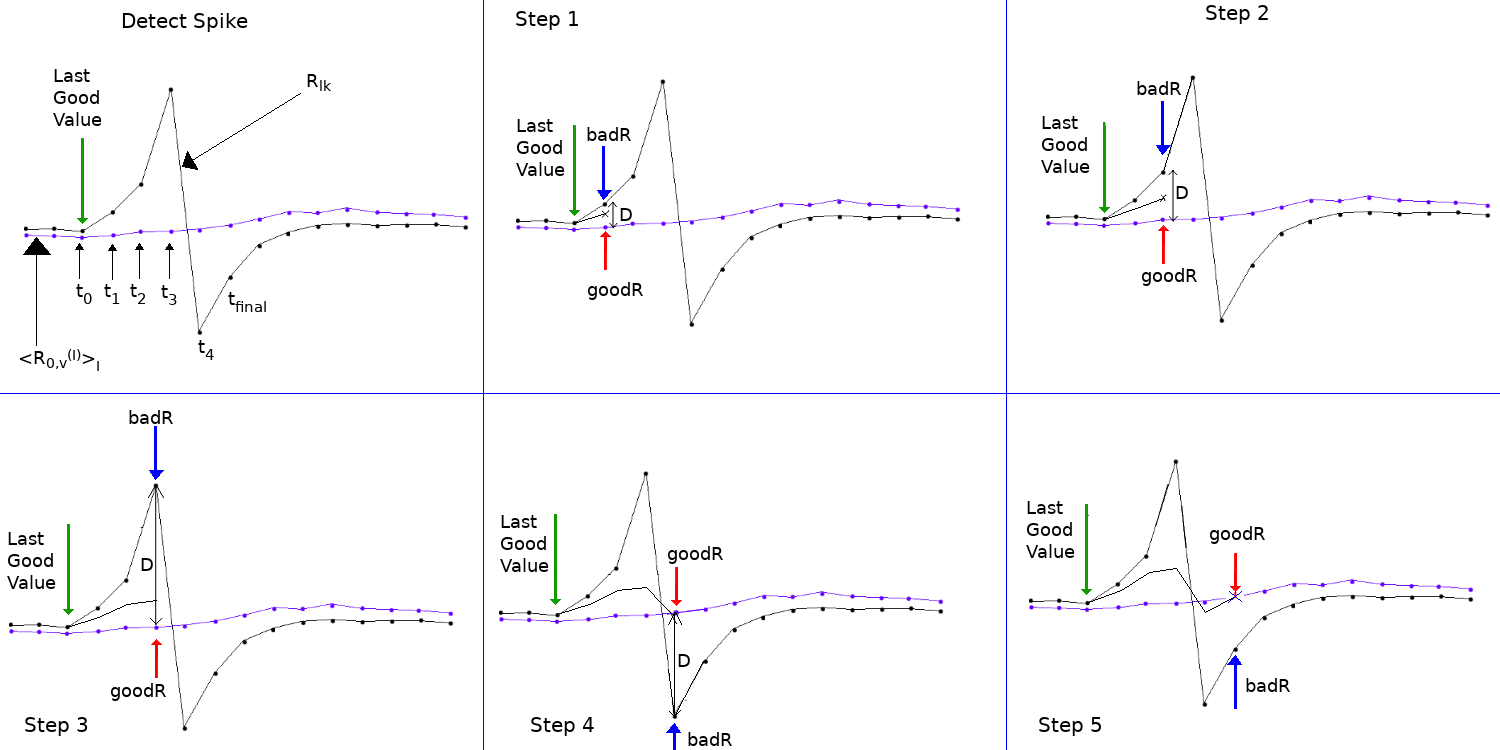
\includegraphics[width=\textwidth]{./img/CTMQC/tanh_explanation.png}
	\caption{\label{fig:tanh_explan}A crude demonstration of the principle behind the smoothing procedure in switching between intercepts. The black line shows an intercept begin to diverge and the alternative intercept is shown in purple. As the step is incremented the amount of the alternative intercept that makes up the effective intercept is increased until only 1 intercept is used.}
\end{figure}


\chapter{Rabi Oscillation \label{ap:Rabi}}
The time dependant Schr\"odinger equation is given below:
\begin{equation}
	i \hbar \frac{\delta}{\delta t} \Phi(\mathbf{R}(t), t) = \hat{H}(\mathbf{R}(t), t) \Phi(\mathbf{R}(t), t)
\end{equation}
If we hold the nuclear coordinates in place (e.g. remove time-dependence from nuclear coordinates) we get an ordinary differential equation as shown below:
\begin{equation}
	i \hbar \frac{d}{d t} \Phi(\mathbf{R}, t) = \hat{H}(\mathbf{R}, t) \Phi(\mathbf{R}, t)
	\label{eq:RABI}
\end{equation}
This has the following general solution. This can be solved with a Taylor series expansion.
\[\Phi(\mathbf{R}, t) = e^{i \hbar \hat{H}t} \Phi(\mathbf{R}, 0)\]
Figure 
\begin{figure}[ht]
  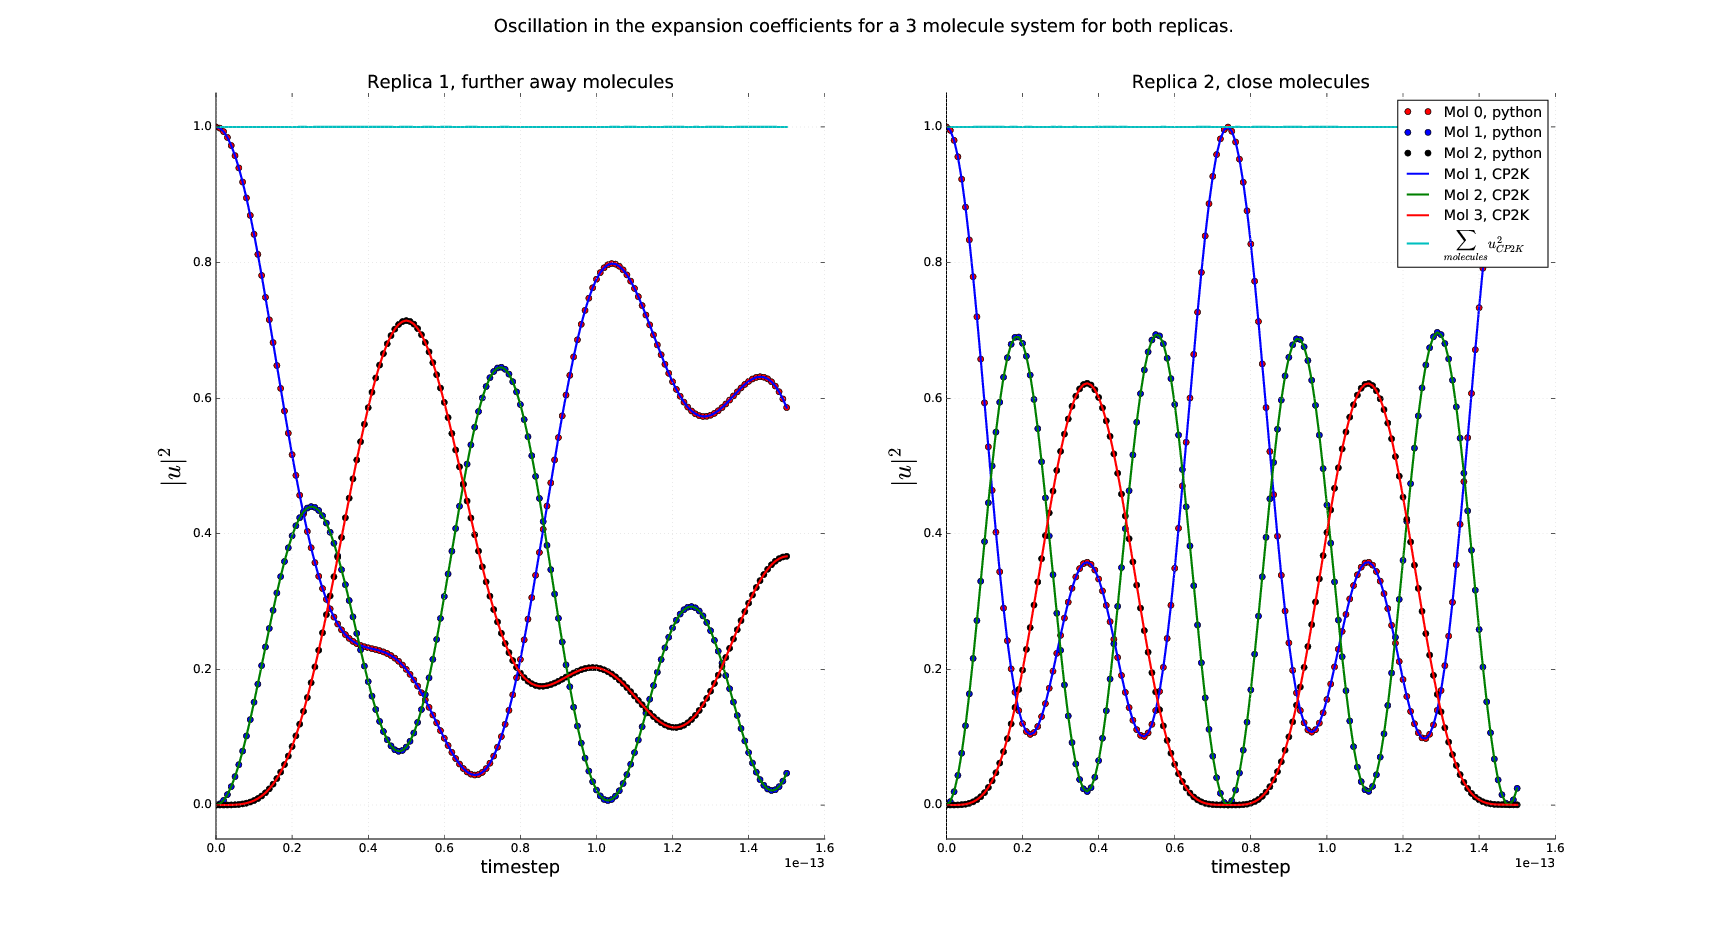
\includegraphics[width=\textwidth]{./img/CTMQC/3_mols_with_python_sol_2_rep.png}
  \caption{\label{fig:Rabi}Rabi oscillation occurring within a Ethylene trimer system. Dotted lines were calculated using equation \eqref{eq:RABI}, solid lines were calculated using the RK4 propagator within the CTMQC section of the CP2K code. The norm is shown on the top as a cyan line and the x axis shows the timestep in seconds.}
\end{figure}









\chapter{Norm Conservation in CTMQC and Ehrenfest}
\label{ap:norm_cons}
A statement of the conservation of the norm, for a single trajectory, is given below in equation \eqref{eq:normConsState}
\begin{equation}
	\frac{d}{dt} \sum_{l} \left\vert C_{l}(t) \right\vert^2 = \sum_{l} C_{l}^{*}(t)\frac{d C_{l}(t)}{dt} + \frac{d C_{l}^{*}(t)}{dt}C_{l}(t)
	\label{eq:normConsState} = 2 \mathbb{R} \left[ \sum_{l} C_{l}(t)^{*} \frac{d C_{l}(t)}{dt} \right]
\end{equation}
Substituting the equation for the evolution of the adiabatic coefficients (and removing the purely imaginary term) into \eqref{eq:normConsState} we get equation \eqref{eq:KsumKadNorm}
\begin{align}
	\frac{d}{dt} \sum_{l} \left\vert C_{l}(t) \right\vert^2 &= 2 \sum_{l} \mathbb{R} \left[ \cancel{\frac{-i}{\hbar} \epsilon_{BO}^{l} C_l(t)^*C_l^{}(t)}
	- \sum_{k} \left[ C_l(t)^*C_k(t) d_{lk}^{ad} - (A_l - B_{l}) C_l(t)^*C_l(t)  \right] \right]
	\\
	&= -2 \sum_{l} \mathbb{R} \left[ \sum_{k} \left[ C_l(t)^*C_k(t) d_{lk}^{ad} - (A_l - B_{l}) C_l(t)^*C_l(t)  \right] \right]
	\label{eq:KsumKadNorm}
\end{align}
Where:
\begin{align}
	A_{l} &= \sum_{\nu = 1}^{N_n} \sum_{k} \frac{\mathcal{Q}_{lk, \nu}(t)}{\hbar M_\nu}\cdot \mathbf{f}_{k, \nu}(t) \vert C_k(t) \vert^2 \ \\
	B_{l} &= \sum_{\nu = 1}^{N_n} \sum_{k} \frac{\mathcal{Q}_{lk, \nu}(t)}{\hbar M_\nu}\cdot \mathbf{f}_{l, \nu}(t) \vert C_{k}(t)\vert^2
\end{align}
The NACE term evaluates to 0 due to the anti-symmetry of the NACE giving us equation \eqref{eq:KsumKadFinalNorm}. 
\\\\
So far, we have proved that the norm should be conserved here for all terms apart from the quantum momentum terms i.e. Ehrenfest.
\begin{align}
	\frac{d}{dt} \sum_{l} \left\vert C^{QM}_{l}(t) \right\vert^2 &= 2 \sum_{l} \mathbb{R} \left[ (A_l - B_{l}) C_l(t)^*C_l(t)  \right] \\
	&= 2 \left[ \sum_l A_l |C_{l}(t)|^2 - \sum_{l} B_{l} \vert C_{l}(t) \vert^2 \right]
	\label{eq:KsumKadFinalNorm}
\end{align}
However, $\sum_{l}A_l |C_{l}|^2 \equiv \sum_{l} B_{l} |C_{l}|^2$, therefore there is no change in the population and the norm should be conserved.
\newpage
%\chapter{Energy Conservation in CTMQC}
%\label{ap:EnerConsDerivation}
%\noindent \textit{Definition:}
%\[\mathbf{A}_{\nu} = \sum_{l} |C_{l}|^2 \mathbf{f}_{l, \nu}  + \hbar \mathbb{I}\left[ \sum_{l, k} C_{l}^{*}C_{k} \mathbf{d}_{\nu, lk} \right]\]
%\begin{align*}
%	\sum_{\nu} \frac{\mathbf{P}_{\nu}}{M_{\nu}} \cdot \mathbf{A}_{\nu} &= \sum_{l, \nu}  |C_{l}|^2 \mathbf{v}_{\nu} \cdot \mathbf{f}_{l, \nu} + \hbar \mathbb{I} \left[ \sum_{l,k, \nu} C_{l}^{*} C_{k} \mathbf{v}_{nu} \cdot \mathbf{d}_{lk, \nu} \right] \\
%	&= \sum_{l, \nu} \mathbf{v}_{\nu} |C_{l}|^2 \mathbf{f}_{l, \nu} + \hbar \mathbb{I} \left[ \sum_{l,k} C_{l}^{*} C_{k} d_{lk} \right] \\
%\end{align*}
%
%
%\begin{align*}
%	\langle \Phi | \dot{\Phi} \rangle &= \langle \sum_{l} C_{l} \psi_{l} | \frac{d}{dt}\left[ \sum_{k} C_{k} \psi_{k} \right] \rangle \\
%	&= \sum_{l} C_{l}^{*} \langle \psi_{l} | \sum_{k} \dot{C}_{k} \psi_{k} + \sum_{k} C_{k} \dot{\psi}_{k} \rangle	\\
%	&= \sum_{l, k} C_{l}^{*}\dot{C}_{k} \langle \psi_{l} | \psi_{k} \rangle + \sum_{l, k} C_{l}^{*}C_{k} d_{lk}	\\
%	&= \sum_{l} C_{l}^{*} \dot{C}_{l} + \sum_{l, k} C_{l}^{*}C_{k} d_{lk} \\
%	&= \mathbb{R}\left[ \sum_{l} C_{l}^{*} \dot{C}_{l} \right] + \mathbb{I}\left[ \sum_{l} C_{l}^{*} \dot{C}_{l} \right] + \sum_{l, k} C_{l}^{*}C_{k} d_{lk} \\
%	&= \frac{1}{2} \frac{d}{dt} \sum_{l} |C_{l}|^2 + \mathbb{I}\left[ \sum_{l} C_{l}^{*} \dot{C}_{l} \right] + \sum_{l, k} C_{l}^{*}C_{k} d_{lk} \\
%	&= \mathbb{I}\left[ \sum_{l} C_{l}^{*} \dot{C}_{l} \right] + \sum_{l, k} C_{l}^{*}C_{k} d_{lk}
%\end{align*}
%
%\begin{align*}
%	\langle \Phi | \hat{H} | \Phi \rangle &= \langle \sum_{l} C_{l} \psi_{l} | \hat{H} | \sum_{k} C_{k} \psi_{k} \rangle \\
%	&= \sum_{l, k} E_{k} C_{l}^{*} C_{k} \delta_{lk} \\
%	&= \sum_{l} E_{l} |C_{l}|^2
%\end{align*}
%

%\begin{align*}
%	E_{pot} &= \langle \Phi | \hat{H} | \Phi \rangle - i\hbar \langle \Phi | \dot{\Phi} \rangle - \sum_{\nu}^{N_{n}} \frac{\mathbf{P}_{\nu}}{M_{\nu}}
% \mathbf{A}_{\nu}
% \\
%  		    &= \sum_{l} E_{l} |C_{l}|^2 - i\hbar \mathbb{I}\left[ \sum_{l} C_{l}^{*} \dot{C}_{l} \right] - i\hbar \sum_{l, k} C_{l}^{*}C_{k} d_{lk} - \sum_{l, \nu} \mathbf{v}_{\nu} |C_{l}|^2 \mathbf{f}_{l, \nu} - \hbar \mathbb{I}\left[ \sum_{l,k} C_{l}^{*} C_{k} d_{lk} \right]
%  \\
%  		    &= \sum_{l} E_{l} |C_{l}|^2 - i\hbar \mathbb{I}\left[ \sum_{l} C_{l}^{*} \dot{C}_{l} \right] - i\hbar \mathbb{I} \left[ \sum_{l, k, \nu} C_{l}^{*}C_{k} \mathbf{v}_{\nu} \cdot \mathbf{d}_{lk} \right] - \sum_{l, \nu} \mathbf{v}_{\nu} |C_{l}|^2 \mathbf{f}_{l, \nu}
%  		    &= \sum_{l} E_{l} |C_{l}|^2 - \sum_{l, \nu} \mathbf{v}_{\nu} |C_{l}|^2 \mathbf{f}_{l, \nu}
%\end{align*}
\chapter{Dynamic $\sigma$ Calculation}
\label{ap:DynamicSigma}
The algorithm for dynamically updating the $\sigma$ parameter outlined in Gossel, 18 \cite{gossel_coupled-trajectory_2018} is provided below.
\begin{enumerate}
  \item Set an initial width parameter ($\sigma_{\nu}^{(I)}(t - dt)$) and a   constant we will name $D$.
  \item Calculate a cutoff distance via: $r_{cut}(t) = D                      \sigma_{\nu}^{(I)}(t - dt)$.
  \item For each atom index, $\nu$, and replica, $I$, gather replicas within  a cutoff distance of the current replica. Set the number of replicas within   the cutoff distance to $N$.
  \item Calculate the distance between atoms on different replicas.
  \item Find the standard deviation of these distances and set the width of   the gaussian, centered on atom $\nu$ and replica $I$, to this standard        deviation.
  \item If the standard deviation is smaller than $\frac{D}{N} min_{I} \left[ \sigma_{\nu}^{(I)} (t - dt) \right]$ then set $\sigma_{\nu}^{(I)}(t) =        \frac{D}{N} min_{I} \left[ \sigma_{\nu}^{(I)} (t - dt) \right]$.
\end{enumerate}

\chapter{Basis Transformation}
\label{ap:BasisTrans}
We can expand the Schr\"odinger equation in terms of a diabatic basis, $\phi$ rather than an adiabatic one, $\psi$. These 2 expansions are given in equations \eqref{eq:SchrodingerAdExpan_ap} and \eqref{eq:SchrodingerDiExpan_ap}.
\begin{equation}
  |\Psi \rangle = \sum_{n} C_{n} | \psi_n \rangle
  \label{eq:SchrodingerAdExpan_ap}
\end{equation}
\begin{equation}
  |\Psi \rangle = \sum_{l} u_{l} | \phi_l \rangle
  \label{eq:SchrodingerDiExpan_ap}
\end{equation}
It follows from this we can define a transformation matrix, $U_{ln}$ to transform between the adiabatic and diabatic bases. This is shown in equation \eqref{eq:TransMat_ap} where the $\overset{\leftrightarrow}{I}$ symbol represents the identity matrix. This identity only holds in the orthogonal diabatic basis $\phi$ and wouldn't hold for non-orthogonal bases.
\begin{equation}
  | \psi_n \rangle = \overset{\leftrightarrow}{I} \left| \psi_{n} \right\rangle = \sum\limits_{l}\left| \phi_{l} \right\rangle \left\langle \phi_{l} \right| \left. \psi_{n}\right\rangle  = \sum_{l} | \phi_{l} \rangle U_{ln}
  \label{eq:TransMat_ap}
\end{equation}
A similar relation between expansion coefficients exists
\begin{align}
  \sum_{n} C_{n} | \psi_{n} \rangle &= \sum_{l} u_l |\phi_{l} \rangle \\
  \sum_{n} C_{n} \langle \psi_{m} | \psi_{n} \rangle &=  \sum_{l} u_l \langle \psi_{m} |\phi_{l} \rangle \\
  C_{m} &=  \sum_{l} u_l U^{*}_{lm}
  \label{eq:ExpansTransMat_ap}
\end{align}
Finally an important property of the transformation matrix is given in equation \eqref{eq:transToDelta}.
\begin{equation}
  \sum_{m} U_{im} U^{*}_{lm} = \sum_{m} \langle \phi_{i} | \psi_{m} \rangle \langle \psi_{m}| \phi_{l}\rangle = \langle \phi_{i} | \phi_{l} \rangle = \delta_{il}
  \label{eq:transToDelta}
\end{equation}
Equations \eqref{eq:TransMat_ap}, \eqref{eq:ExpansTransMat_ap} and \eqref{eq:transToDelta} will be used below to transform the propagation equations from the adiabatic basis to the diabatic one.

\label{chap:basisTrans}
\section{Forces}
\label{sect:ad2di_frc}
The equation for the propagation of the forces in the adiabatic basis is:
\begin{align}
  \begin{split}
      \mathbf{F}_{\nu}^{(I)} = &- \sum_{n} |C_{n}^{(I)}|^2                    \nabla_{\nu}E_{n}^{(I)} - \sum_{n, m} C_{m}^{* (I)} C_{n}^{(I)}               \left(E_{n}^{(I)} - E_{m}^{(I)} \right) \mathbf{d}_{\nu, mn}^{ad, (I)} \\
      &- \sum_{m, n} |C_{m}^{(I)}|^2 \left( \sum_{\nu'}^{N_{n}} \frac{2}{\hbar   M_{\nu'}} \mathcal{Q}_{\nu', mn}^{(I)} \cdot \mathbf{f}_{m, \nu'}^{(I)}       \right)\left[ \mathbf{f}_{n, \nu}^{(I)} -            \mathbf{f}_{m, \nu}^{(I)} \right] |C_{n}^{(I)}|^2 
  \end{split}
  \label{eq:adForce_ap}
\end{align}
The quantum momentum part of the equation cannot be easily transformed so this will focus on the Ehrenfest part:
\begin{equation}
  \mathbf{F}_{eh, \nu}^{(I)} = - \sum_{n} |C_{n}^{(I)}|^2 \nabla_{\nu}E_{n}^{(I)} - \sum_{n, m} C_{m}^{* (I)} C_{n}^{(I)} \left(E_{n}^{(I)} - E_{m}^{(I)} \right) \mathbf{d}_{\nu, mn}^{ad, (I)}
  \label{eq:adForceEhren_ap}
\end{equation}
Using equation (10) in Carof, 17 \cite{carof_detailed_2017} and the Hellman-Feynman theorem we can rewrite equation \eqref{eq:adForceEhren_ap} as equation \eqref{eq:adForceReduce_ap}:
\begin{equation}
  \mathbf{F}_{eh, \nu}^{(I)} = \sum_{m, n} C_{m}^{* (I)} C_{n}^{(I)} \langle \psi_{m} | \nabla_{\nu} H | \psi_{n} \rangle
  \label{eq:adForceReduce_ap}
\end{equation}
We can substitute the coefficients and basis functions for those in equations \eqref{eq:TransMat_ap} and \eqref{eq:ExpansTransMat_ap}. This carried out in equation \eqref{eq:transProc_ap}. However, I have removed the trajectory and atom index from the terms to make the notation clearer.
\begin{align}
  F_{eh, \nu} &= \sum_{m, n} C^{*}_{m} C_{n} \langle \psi_{m} | \nabla_ H | \psi_{n} \rangle \\
  &= \sum_{m, n} \sum_{i} u_i^{*} U_{im} \sum_{j} u_j U^{*}_{jn} \sum_{l}U_{lm}^{*} \sum_{k} U_{kn} \langle \phi_{l} | \nabla H | \phi_{k} \rangle \\ 
  &= \sum_{m, n} \sum_{i, j, k, l} u_i^{*}  u_j U_{im} U_{lm}^{*} U^{*}_{jn} U_{kn} \langle \phi_{l} | \nabla H | \phi_{k} \rangle \\ 
  &= \sum_{i, j, k, l} u_i^{*}  u_j \delta_{il} \delta_{jk} \langle \phi_{l} | \nabla H | \phi_{k} \rangle \\ 
  &= \sum_{i, j} u_i^{*}  u_j \langle \phi_{i} | \nabla H | \phi_{j} \rangle 
  \label{eq:transProc_ap}
\end{align}
However, in the code the expectation value of the gradient of the Hamiltonian ($\langle \phi_i | \nabla H | \phi_j \rangle$) isn't very easily calculable. However, the gradient of the Hamiltonian matrix elements ($\nabla \langle \phi_i | H | \phi_j \rangle$) is easily calculable via the overlap term, $\nabla H = C \nabla S_{ij}$. Therefore, using chain rule we can re-write equation \eqref{eq:transProc_ap} as:
\begin{align}
  F_{eh, \nu} &= \sum_{i, j} u_i^{*}  u_j \langle \phi_{i} | \nabla H | \phi_{j} \rangle \\
  &= \sum_{i, j} u_i^* u_j \left(\nabla \langle \phi_i| H | \phi_j \rangle - \langle \nabla \phi_i| H | \phi_j \rangle - \langle \phi_i| H | \nabla \phi_j \rangle \right) \\
  &= \sum_{i, j} u_i^* u_j \left(\nabla \langle \phi_i| H | \phi_j \rangle - \sum_{l}\langle \nabla \phi_i| \phi_l \rangle \langle \phi_l | H | \phi_j \rangle - \sum_l \langle \phi_i| H | \phi_l \rangle \langle \phi_l | \nabla \phi_j \rangle \right) \\
  &= \sum_{i, j} u_i^* u_j \left(\nabla \langle \phi_i| H | \phi_j \rangle + \sum_{l}\mathbf{d}_{il} \langle \phi_l | H | \phi_j \rangle - \sum_l \mathbf{d}_{lj} \langle \phi_i| H | \phi_l \rangle \right)
\end{align}

\noindent Giving the final equation for the transformed forces as:
\begin{equation}
  \mathbf{F}_{eh, \nu}^{(I)} = \sum_{i,j} \mathbf{u}_{i}^{*(I)} \mathbf{u}_{j}^{(I)} \left( \nabla_{\nu} H_{ij}^{(I)} + \sum_{l} \mathbf{d}_{lk, \nu}^{(I)} H_{lj}^{(I)} - \sum_{l} \mathbf{d}_{lj, \nu}^{(I)} H_{il} \right)
  \label{eq:ForceDiab_ap}
\end{equation}

\chapter{Adiabatic State Initialisation}
\label{ap:AdiabaticSelector}
By diagonalising the Hamiltonian we get the adiabatic energies (eigenvalues) for each state and transformation matrix (eigenvectors) to calculate diabatic states $\mathbb{U}$. We can calculate diabatic coefficients corresponding to each adiabatic state via equation \eqref{eq:CtoU_trans} below.
\begin{equation}
	\mathbb{U} \mathbf{C}_{n} = \mathbf{u}_{n}
	\label{eq:CtoU_trans}
\end{equation}
Where $\mathbb{U}$ is the transformation matrix of size (N$_{\text{mol}}$,  N$_{\text{mol}}$), $\mathbf{C}$ is a complex vector of size N$_{\text{mol}}$ containing coefficients for adiabatic state n and $\mathbf{u}$ is a complex vector of size N$_{\text{mol}}$ containing coefficients for diabatic state n.
\\\\
Seeing as we would like to find the diabatic population corresponding to each adiabatic state we localise coefficients on each pure adiabatic state and carry out the transformation e.g: $C_i = (1+0i, 0+0i, 0+0i, ...)$ when we want to find the diabatic coefficient corresponding to state 1 and $C_i = (0+0i, 1+0i, 0+0i, ...     )$ when we want to find the diabatic coefficient corresponding to state 2 etc.. Therefore, the column, n, of the transformation matrix, $\mathbb{U}$, gives the diabatic coefficients corresponding to adiabatic state, n, as shown below in equation \eqref{eq:trans_equal_u}
\begin{equation}
	U_{in} = u_{i}
	\label{eq:trans_equal_u}
\end{equation}
Where n is the adiabatic state index and i is the diabatic (molecular) state index.
\\\\
Once we have the diabatic state corresponding to each adiabatic state, and the energy of that adiabatic state, we can find which state best fulfills the requirements of being close to the center of the system and being within 3KT of the ground state. In order to do this, we can loop over each adiabatic state in increasing order of energy. The center of the system is calculated and the population weighted average center of mass, $\mathbf{R}_n$ of the diabatic coefficients corresponding to adiabatic state n is calculated as in equation \eqref{eq:COM_pop}.
\begin{equation}
	\mathbf{R}_{n} = \sum_{i} |u_{i}|^2 \mathbf{R}_{COM, i}
	\label{eq:COM_pop}
\end{equation}
The Euclidean distance between the center of the system and $\mathbf{R}_{COM, i}$ is calculated and if this distance is below some threshold value then we initialise the surface hopping trajectory on that adiabatic state. If we do not find any states within 3KT of the ground state and within an acceptable radius of the center we start again this time increasing the maximum allowed distance from the center. If this maximum allowed distance is increased such that we reach another threshold distance the energy threshold is increased this time until a state is found that is close enough to the center. In this way we find an adiabatic state, which when transformed, gives a diabatic population close to center of the system and near the ground state energy.



\chapter{Center of Mass Restraints}
\label{ap:Restraints}
\begin{wrapfigure}{r}{0.38\textwidth}
    \vspace*{-0.7cm}
    \centering
    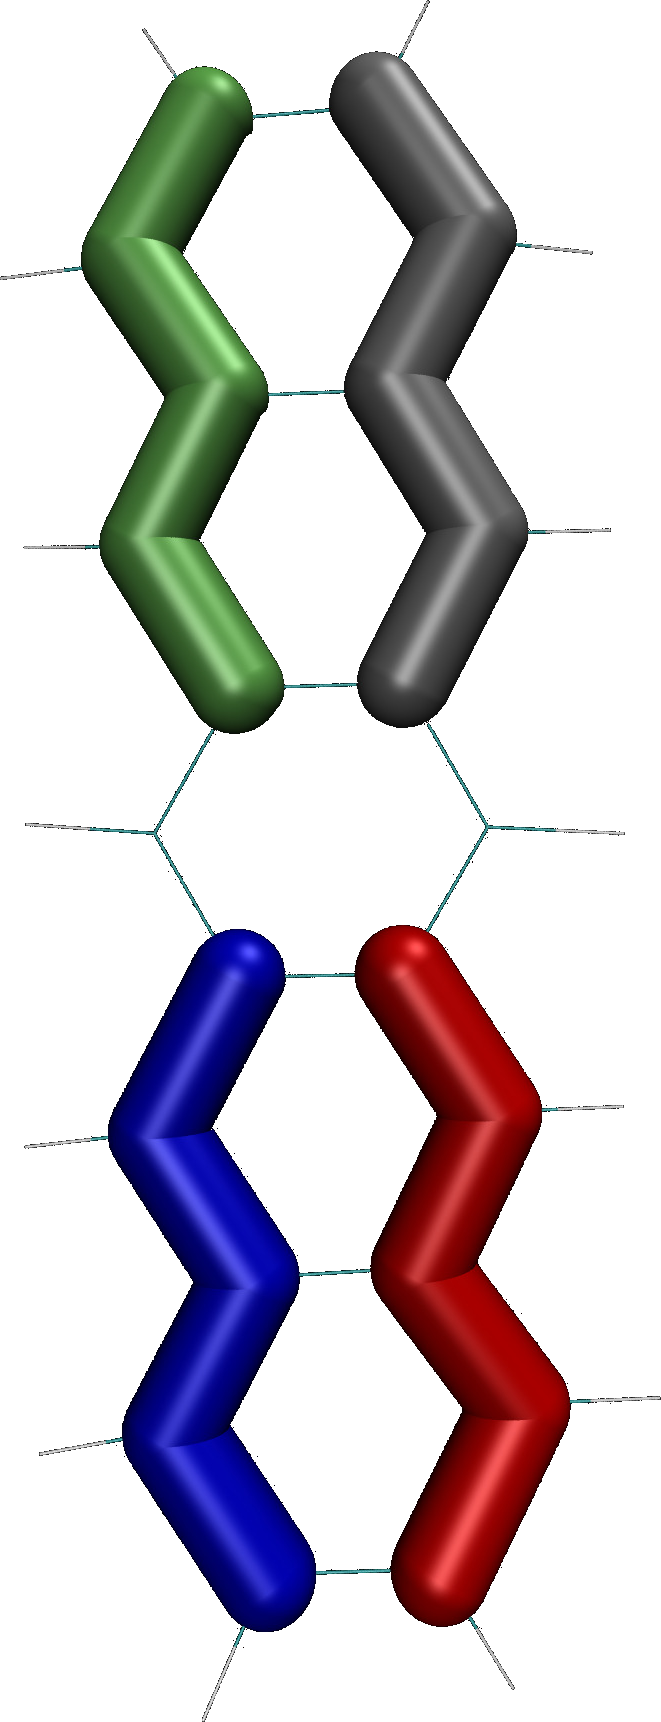
\includegraphics[width=0.14\textwidth]{./img/RestraintsPos.png}
    \caption{\label{fig:rest}The restraint set up for 1 molecule. Each coloured zig-zag shows the atoms that are restrained.}
\end{wrapfigure}
The surface hopping code at the time did not support electrostatic interactions. So, in order to maintain the structure from the molecular dynamics simulations, center of mass restraints were used on each molecule. The restraint set up for 1 molecule is shown in figure \ref{fig:rest}. Here each of the 4 coloured zig-zag shapes show which atoms are restrained. These atoms were restrained about their center of mass. This configuration of restraints was used in order to stop rotations about the long axis for each molecule as this would allow molecules to form a face-to-face stacking giving rise to unphysically high couplings. The restraint strength was chosen to be the same as in another group members study to allow for a fair comparison of  results. A short MD equilibration was performed to determine whether the restraint spring constant was sufficient to hold the molecules in place well enough to prevent the very high couplings appearing in the global coupling    distribution. To further validate the choice of restraint/general set up a surface hopping simulation was carried out on a layer of bulk crystal and the mobilities were compared to known values.

\chapter{Active Systems}
\label{ap:system_divisions}

\section{0ns and 1ns Systems}
\begin{figure}[ht]
	\includegraphics[width=\textwidth]{./img/DifferentQuenchTimes/0ns/0nsSubsystems.png}
	\caption{\label{fig:0nsSubSys}Panel a) shows a system chosen to run surface hopping on, molecules in gray are fixed in place blue molecules show the active region. Panel b) shows every substructure chosen in the 0ns quenched structure.}
\end{figure}
The selection of the region for each surface hopping simulation was important in order to get a fair representation of the mobilities achievable within each structure. In the 0ns and 1ns quenched structures 6 slices were selected from the final snapshot of the structure. These were chosen to be independent clusters evenly spaced to sample the mobility of the structure at various points. The selections are shown in figure \ref{fig:0nsSubSys} for the 0ns quenched structure. The same process was used in the 1ns quenched structure.
\\\\
In order to preserve the structure and maintain energy conservation a shell of inactive molecules was selected from the superstructure to surround the active region. The atoms within this remained fixed to their position at t=0.
\section{100ns System}
\begin{figure}[ht]
	\centering
	\includegraphics[width=\textwidth]{./img/DifferentQuenchTimes/100ns/AllClusters_labelled.png}
	\caption{\label{fig:100nsClusteredLabelled}The 100ns quenched structure clustered by layer. Each different colour represents a different cluster, labelled with the numbers around the edge of the structure.}
\end{figure}
The 100ns system is a much more ordered system and forms very well defined layers. This makes picking out structures on which to run surface hopping different to the 0/1ns quenched structures. The method I used was to first extend the superstructure in the z axis by $\pm45 \angstrom$ by repeating the periodic image and discarding molecules more than $\pm45 \angstrom$ from the simulation box boundaries. This was to ensure the resulting system was sufficiently large to converge mobilities. This added approximately 1 extra periodic image in the $+^{\text{ve}}$ and $-^{\text{ve}}$ z direction. A density based clustering algorithm (similar to DBSCAN \cite{DBSCAN}) was used to isolate the layers in the full structure by clustering centers of mass. These are shown in figure \ref{fig:100nsClusteredLabelled}. In this figure clusters 6, 7 and 11 were chosen to calculate the mobility via surface hopping.

\section{10ns System}
\begin{wrapfigure}{r}{0.45\textwidth}
	\includegraphics[width=0.45\textwidth]{./img/DifferentQuenchTimes/10ns/Clusters.png}
	\caption{\label{fig:10nsClusters}The clusters chosen to run surface hopping simulations on. The coloured clusters each represent a different structure on which surface hopping was ran.}
\end{wrapfigure}
The choice of region within the 10ns quenched structure was different from the 0/1ns and the 100ns quenched structure. Here we have some large crystal fragments forming but still very few well defined layers. In this system the mobility is expected to be much more dependant on the initial position of the charge carrier within the structure than in the 0ns and 100ns quenched structure where the structure was more uniformly disordered or ordered respectively. In order to sample a reasonable range of mobilities in this structure 4 clusters were selected shown in fig \ref{fig:10nsClusters}. 3 of these (red, blue and purple) were selected using a similar clustering procedure as in the 100ns quenched structure. The center-right green cluster was selected as it looked like it was a fairly disordered region where multiple crystal fragments meet, which would give a lower bound on the mobility within the 10ns structure.

\chapter{Additional Pentacene Mobility Information}
\label{ap:PentTable}
\begin{figure}[htbp]
%\begin{table}
	\caption{\label{tab:ap:expCompPent}Experimental and computed charge mobilities for amorphous, polycrystalline and single-crystalline pentacene.}
	\label{}
	%\begin{center}
{\footnotesize
\hspace*{-2.8cm}
		\begin{tabular}{lllllll}
			Author & device/comp.  & structure & gate dielectric & mobility & comments  \\
			\hline \\
			1, Hesse80 & Photocurrent  & amorphous &             &  0.001-0.01 & long time mobility (1 $\mu$s)     \\
			2,               &                                                      &                    & & 0.4  & short time mobility (20 ns)   \\
			3, Bae13 & TFT  & amorphous & polymer & 0.04-0.14 & dependent on deposition rate \\
			4, Choo02 & TFT  & amorphous & SiN$_x$/p-Si & 0.3 &  \\
			5              &                             & amorphous-crystalline &  & 0.1 &   \\
			6, this work &   comp.     & amorphous &  & 0.2 &  bulk, 0\% crystallinity \\
			              \hline \\
			7, Knipp04 & TFT  & polycrystalline &  SiN$_3$ & 0.2-0.55 & grain size 3-7 $\mu$m \\
			8                   &         & polycrystalline & thermal SiO$_2$+OTS & 0.5-1.4 & grain size 1-2 $\mu$m \\
			9, Fritz05  & TFT & polycrystalline    & SiO$_2$ rough      & 0.02   & \\
			10                  &        &                             & SiO$_2$ smooth  &  0.31  & \\
			11                  &        &                        &  SiO$_2$+polymer & 0.62 & \\
			12, Duffy08 & TFT & polycrystalline &  SiO$_2$+BCB & 0.4-0.7 & large crystals \\
			13, Klauk02 & TFT & polycrystalline & SiO$_2$ & 0.4 &  \\
			14                    &       &                         & SiO$_2$+OTS  &  1.0      &      \\
			15                  &       &                         & Si+polymer   &  3.0   &         \\
			16,  this work &   comp.        & nanocrystalline &  & 0.2 & bulk, 30\% crystallinity \\
			17,  this work &   comp.        & nanocrystalline &  & 0.9 & bulk,  60\% crystallinity \\
			18,  this work &   comp.       & nanocrystalline &  & 1.8 & bulk, 80\% crystallinity \\
			\hline \\
			19,   Zhang16 & OFET & 2D single crystal & boronitride &  1.6 & monolayer (1L)  \\
			20,  this work &   comp.        & 2D single crystal &   & 4.2 & monolayer (1L) \\
			21,  Zhang16 & OFET & 2D single crystal & boronitride &  3 & bilayer (2L)  \\
			22,  this work &   comp.        & 2D single crystal &   & 7.3  & bilayer (2L) \\
			\hline \\
			23, Lee06 & OFET & single crystal & SiO$_2$ & 2.3 & largest, polymorph unknown \\
			24, &  &  & & 0.66 & smallest, polymorph unknown \\
			25, Takeyama12 & OFET & single crystal & Al$_2$O$_3$+ionic liquid & 5 & polymorph I, crystal size 200 $\mu$m \\
			26,  Arabi16 & OFET &  single crystal & SiO$_2$ & 5.6 & crystal size 50 $\mu$m \\
			27,  this work &   comp.        &  single crystal &   & 10.5 & bulk, polymorph I \\
		\end{tabular}
}
	%\end{center}
%\end{table}
\end{figure}


\chapter{Addition-Subtraction Forces}
\label{ap:EwaldForcesAddSub}
\section{Real Space}
The real space forces in the addition subtraction scheme are given in equation \eqref{eq:AddSubForcesReal}.
\begin{equation}
  \mathbf{F}_{i}^{\gamma} = \left\lbrace \begin{array}{lc} \mathbf{F}_i^{N}(\mathbf{R}) + \sum_{j \in \gamma} (q_i^{C} q_j^C - q_{i}^N q_j^{N}) \mathbf{f}_{ij}(\mathbf{R}) + \sum_{j \notin \gamma} (q_i^{C} q_j^{N} - q_{i}^N q_j^{N}) \mathbf{f}_{ij}(\mathbf{R}); & i \in \gamma \\\\
\mathbf{F}_i^{N}(\mathbf{R}) - \sum_{j \in \gamma} (q_i^{C} q_j^N - q_{i}^N q_j^{N}) \mathbf{f}_{ij}(\mathbf{R}); & i \notin \gamma
\end{array} \right.
  \label{eq:AddSubForcesReal}
\end{equation}
Where:
\begin{itemize}
  \item $\mathbf{f}_{ij}(\mathbf{R}) = \frac{\hat{\mathbf{R}}_{ij}}{|\rij|} \left(\frac{erfc\left(\alpha |\rij| \right)}{|rij|} + \frac{2 \alpha}{\sqrt{\pi}} e^{-\alpha^2 |\rij|^2} \right)$: the force between atoms i and j.
  \item $\mathbf{F}_i^{N}(\mathbf{R}) = q_i^{N} \sum_{j}^{N_{at}} q_j^N \mathbf{f}_{ij}(\mathbf{R}) $: the total neutral force.
  \item $q_{j}$ is the charge on atom j
  \item $\gamma$ is the index of the charged molecule.
\end{itemize}
Once again, we first calculate the total force between all neutral molecules. The charge-charge interactions are substituted in for the neutral-neutral interactions for atoms on the charged molecule. The charge-neutral interactions are then substituted in for the neutral-neutral interactions for the charged molecule and its environment. The bonded interaction corrections are the same as these.

\section{Reciprocal Space}
\label{ap:EwaldForcesAddSubRecip}
The reciprocal space forces, as mentioned in the main text, cannot be decomposed with the addition-subtraction scheme.

\begin{equation}
	\F_{i}^{\gamma}(\mathbf{R}) =  \left\lbrace \begin{array}{lc}
	  4\pi q_{i}^{C} \sum_{\mathbf{k} \neq 0} \mathrm{Im}\left[ S^{'}_{\mathbf{k}} E_{\mathbf{k},i}^{*} \right]; & i \in \gamma\\\\
	
	4\pi q_{i}^{N} \sum_{\mathbf{k} \neq 0} \mathrm{Im}\left[ S^{'}_{\mathbf{k}} E_{\mathbf{k},i}^{*} \right];& i \notin \gamma
	\end{array}
	\right.
	\label{eq:AddSubForcesRecip}
\end{equation}
Where:
\begin{itemize}
  \item $S_{\mathbf{k}}^{'} = A_{\mathbf{k}} \left[\sum_{j} q_j^{N} E_{\mathbf{k}, j} + \sum_{j \in \gamma} \left(q_j^{C} - q_{j}^{N}\right) E_{\mathbf{k}, j}\right]$

  \item $A_{\mathbf{k}} = \frac{\mathbf{k}}{|\mathbf{k}|^2} e^{\frac{|\mathbf{k}|^2}{4 \alpha^2}}$

  \item $E_{\mathbf{k}, j} = e^{2 \pi \mathrm{i} \mathbf{k} \cdot \R_{j}}$
\end{itemize}
\noindent The calculation of this equation scales as $\mathcal{O}(N^3)$ where $N^3 = N_{states} N_{at} N_{k}$. This is because for every atom, $i$, in charged molecule, $\gamma$, a loop over $\mathbf{k}$ vectors must be calculated.

\chapter{Colophon}
\label{appendixlabel3}
This document was set in the Times Roman typeface using \LaTeX (specifically LuaTeX) and Bib\TeX + make, composed with Vim.
